\documentclass{beamer}
\usepackage{amsmath,hyperref}

\usetheme{boxes}

\usepackage{Sweave}
\begin{document}
\Sconcordance{concordance:moz-model-pres.tex:moz-model-pres.Rnw:%
1 14 1 1 0 25 1 1 13 1 2 267 1}

\title{Slightly Less Simple Mosquito Modeling}
\author[Pearson]{Carl~A.~B.~Pearson}
\institute[University of Florida]{
Emerging Pathogens Institute, University of Florida
}
\frame{\titlepage}

\frame{
\frametitle{What's this talk really about?}
\begin{itemize}
\item expression with models,
\item simple analytical approaches,
\item a little dimensional analysis,
\item how to connect those with experiments, and
\item a little about work habits and tools
\end{itemize}
}

\frame{

\begin{figure}
\begin{center}
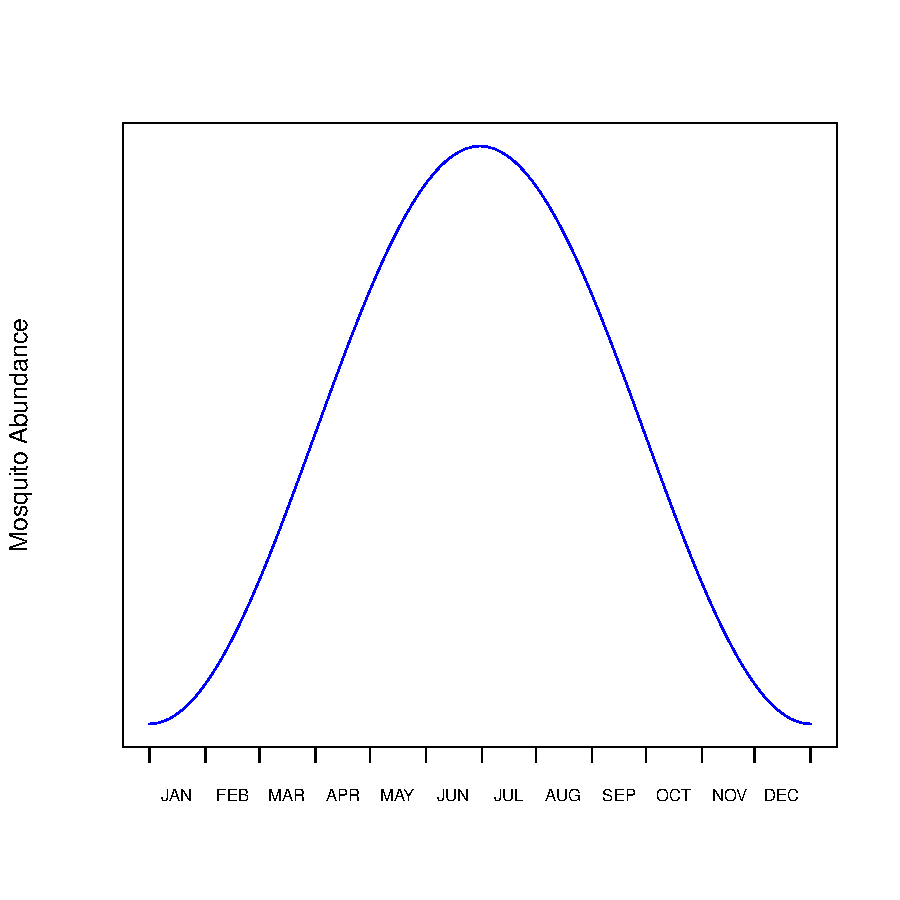
\includegraphics{moz-model-pres-plotfig1}
\end{center}
\end{figure}

}

\frame{

\begin{figure}
\begin{center}
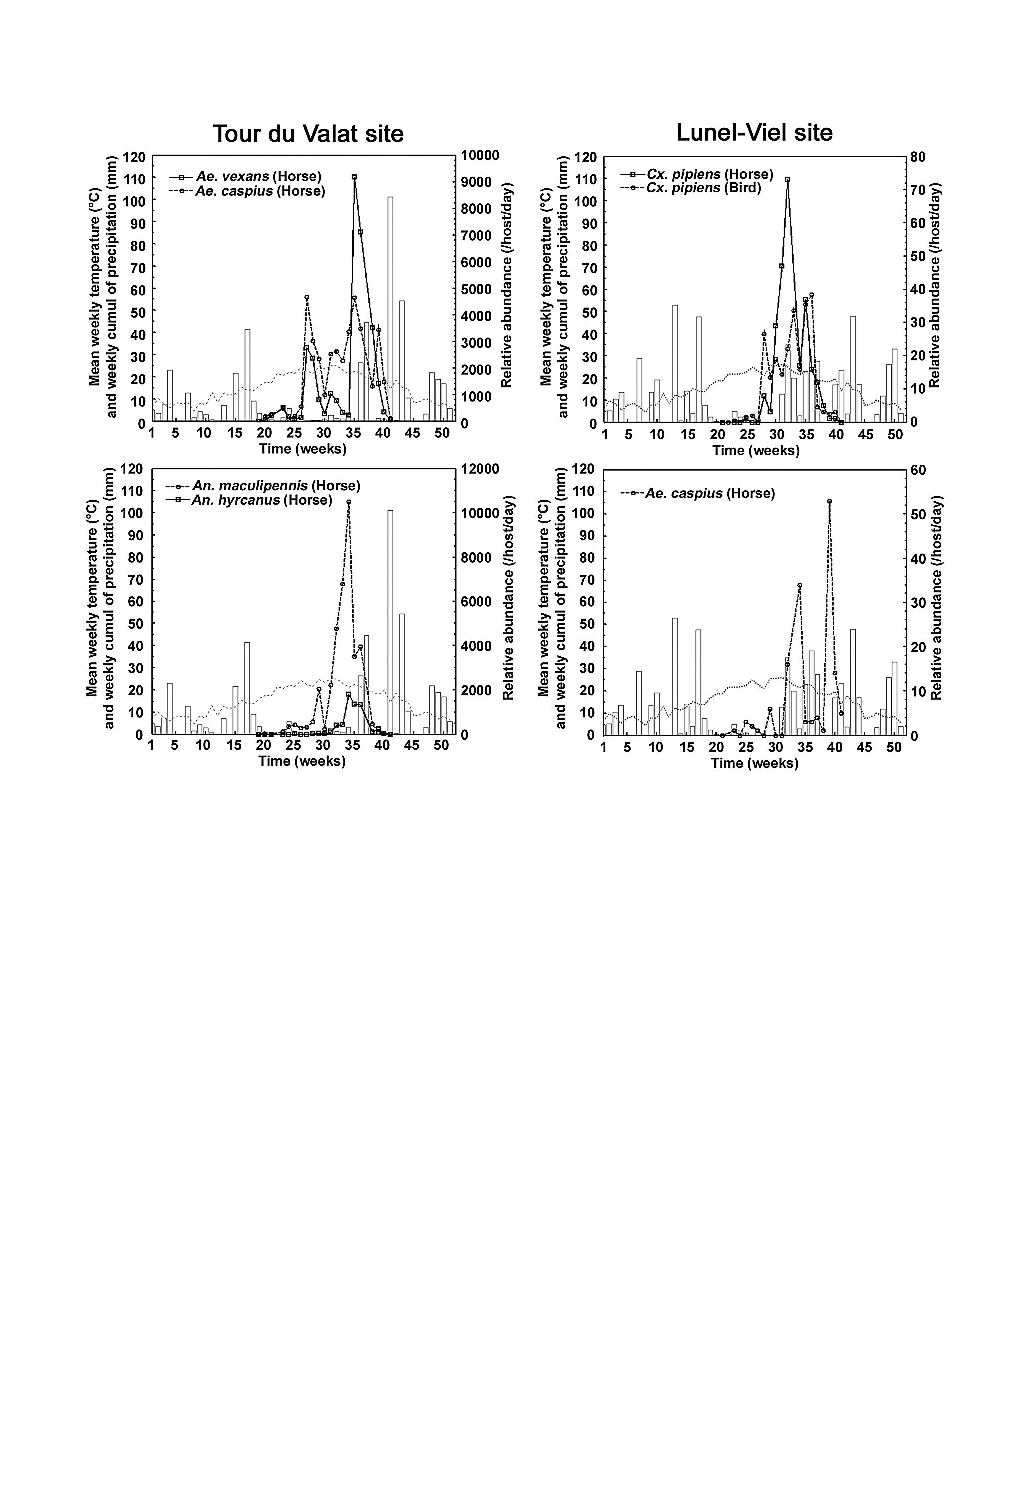
\includegraphics[width=0.8\textwidth]{insert.pdf}
\caption{Bicout et al. "Horse-, Bird-, and Human-Seeking Behavior and Seasonal Abundance of Mosquitos in a West Nile Virus Focus of Southern France". J. Med. Entomol. 43(5): 936-946 (2006)}
\end{center}
\end{figure}

}

\frame{
\frametitle{So, a Disconnect.}
Specifically, it is impossible to match features like peak population, total population over a year, and turnover rate with a functional form

$$
M(t) = C\sin(\omega t+\theta)
$$

\ldots and these features can be critical to predicting transmission dynamics, and thus planning interventions.
}

\frame{
\frametitle{Do Better, But Keep It Simple}
What's appealling about this trigonometric representation?  Simplicity:

\begin{itemize}
\item two parameters
\item no spatial features
\item ``easy'' analytical form
\end{itemize}

Possible to identify alternatives that {\em can} match salient features, but still retain these features?
}

\frame{
What are those salient features?
}

\frame{
\begin{itemize}
\item every year,
\item over a relatively short duration,
\item the mosquito population rapidly increases,
\item sits at a high level of activity,
\item then rapidly declines,
\item apparently connected with resource availability \&\ environmental suitability
\end{itemize}
}

\frame{
What's present in the trigonometric formulation?
\begin{itemize}
\item every year, {\bf CHECK!} \ldots {\em but not the rest of:}
\item over a relatively short duration,
\item the mosquito population rapidly increases,
\item sits at a high level of activity,
\item then rapidly declines,
\item apparently connected with resource availability \&\ environmental suitability
\end{itemize}
}

\frame{

}


\frame{
\title{Engineering \&\ Maths Refresher, I}
\begin{enumerate}
\item useful to write models in terms of measurable parameters,
\item measurable parameters are not scale-free,
\item mathematics is more useful when scale free, therefore
\item dimensional analysis is awesome
\end{enumerate}
}

% \frame{
% where $M(t)$ is mosquito population w.r.t time
% \begin{align*}
% \dot{M(t)} = E(t) - \lambda M(t)
% \end{align*}
% defined on $t\in(-T/2,T/2)$
% }
% 
% \frame{
% common usage is $M(t)\propto$ simple trigonometric
% 
% What salient observed features does that miss?
% 
% aside: why replace given $M(t)$ with given $\dot{M(t)}$?
% }
% 
% \frame{
% Salient features:
% \begin{itemize}
% \item short time with appreciable population
% % note: measure of pop. may be totally unreliable; however, trappable pop might good surrogate for active pop.
% \item even shorter time for population rise and fall
% \item low correlation with early and peak populations % accurate? provide comparison plots?
% \end{itemize}
% 
% Need a spike-like $E(t)$ to replicate these.  Candidates?
% }
% 
% \frame{
% Spike-like could be more formally $\delta$-function like.
% 
% So: use $\delta$-function approximations.
% }
% 
% \frame{
% TODO list approximate delta functions.
% }
% 
% \frame{
% What should we use for the shape parameters?
% 
% clue: want oranges-to-oranges comparisons between the options
% }
% 
% \frame{
% I chose to make mosquito total births equivalent
% 
% TODO $M_p$ equation
% 
% and then to apply a subjective ``constraint'' on $\Delta t$
% 
% TODO delta t stuff
% }
% 
% \frame{
% TODO list approximate delta functions with params in place
% }
% 
% \frame{
% Now everything is on the same scale, but rewind: don't have any of the convenience of having the same scale.
% 
% So: dimensional analysis.  What parameters should be eliminated?
% }

\frame{
\frametitle{``New'' Habits and Tools}
The general arrow of scientific work has been towards increased specialization and collaboration.

This presents a few challenges to getting work done:
\begin{itemize}
\item lashing together methods from different fields,
\item getting genuine peer-review, and
\item the purely mechanical handling of different people simultaneously working on the same ``thing''
\end{itemize}

How can we address these issues?
%.  The final specialist work product can be very intimidating to collaborators with other specialities, which can make a collaboration's skeptical review of their combined product difficult. That's on top of the pure mechanics of handling multiple people modifying the same ``thing''.
% I come from a background where all collaborators are responsible for the entire product, not just their narrowly focused piece
}

\frame{
\frametitle{``New'' Habits and Tools}
Fortunately, there's a whole industry that's continuously tackling this exact problem: software development, and more specifically open-source software projects.

What tools and habits can we adopt from this field?  What risks are associated with that?  What's still missing?
}

\frame{
\frametitle{The Good}
\begin{itemize}
\item version control systems,
\item collaborative tools on top of those,
\item preference for code documentation leading to
\begin{itemize}
\item bite-sized parts,
\item modularity,
\item re-usability, and
\item verifiability (a/k/a unit testing)
\end{itemize}
\item open availability of all source,
\item combines with version control to provide complete history of work product
\end{itemize}
}

\frame{
\frametitle{The Bad}
\begin{itemize}
\item openness can make for opportunity to be ``scooped'',
\item can focus more on process than product,
\item learning curve for most scientists
\end{itemize}
}

\frame{
\frametitle{The Ugly}
\begin{itemize}
\item university contracts' intellectual property clauses,
\item academic institutions don't ``get'' these tools,
\item community adoption?
\end{itemize}
}

\frame{
\frametitle{Why bring this up?}
It's a little bit advocacy, and \href{https://github.com/pearsonca/moz-model-pres}{I built this presentation using this work model.}
}

\end{document}
